\documentclass[tikz,border=8pt]{standalone}
\usepackage{amsmath,amssymb}
\usetikzlibrary{arrows.meta,automata,positioning,quotes}
\begin{document}
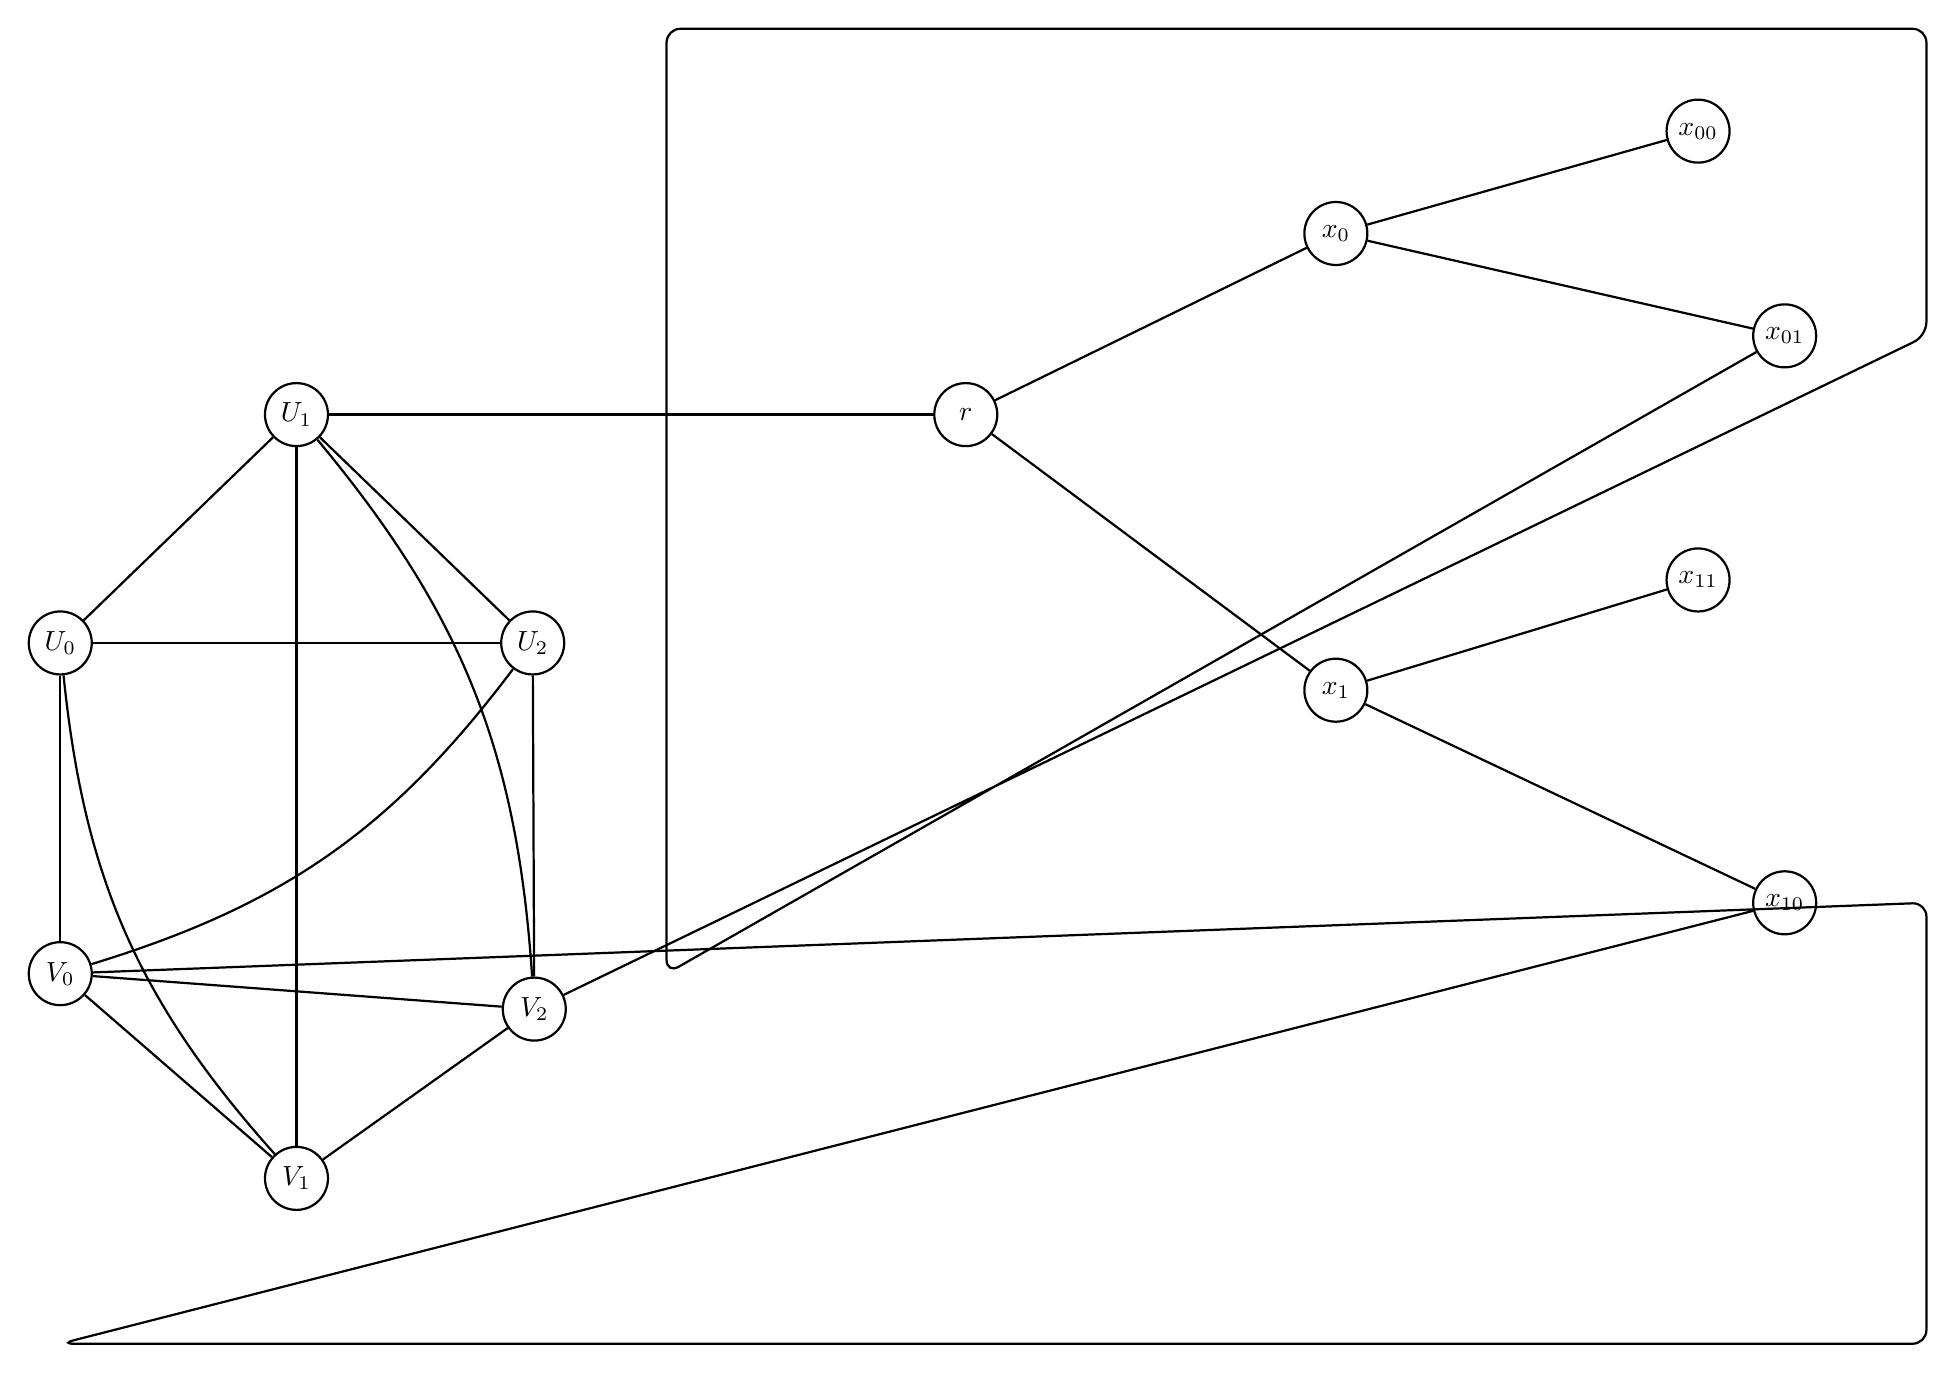
\begin{tikzpicture}[x=1cm,y=1cm]
\tikzset{
  graphnode/.style={circle,draw,thick,minimum size=8mm,inner sep=1pt,font=\sffamily},
  directed/.style={-{Stealth[length=2.4mm]},thick},
  undirected/.style={thick}
}
\node[graphnode] (n_U0) at (-12.00,1.60) {$U_0$};
\node[graphnode] (n_U1) at (-9.00,4.50) {$U_1$};
\node[graphnode] (n_U2) at (-6.00,1.60) {$U_2$};
\node[graphnode] (n_V0) at (-12.00,-2.60) {$V_0$};
\node[graphnode] (n_V1) at (-9.00,-5.20) {$V_1$};
\node[graphnode] (n_V2) at (-5.98,-3.05) {$V_2$};
\node[graphnode] (n_r) at (-0.50,4.50) {$r$};
\node[graphnode] (n_x0) at (4.20,6.80) {$x_0$};
\node[graphnode] (n_x1) at (4.20,1.00) {$x_1$};
\node[graphnode] (n_x00) at (8.80,8.10) {$x_{00}$};
\node[graphnode] (n_x01) at (9.90,5.50) {$x_{01}$};
\node[graphnode] (n_x10) at (9.90,-1.70) {$x_{10}$};
\node[graphnode] (n_x11) at (8.80,2.40) {$x_{11}$};
\draw[undirected] (n_U0) -- (n_U1);
\draw[undirected] (n_U1) -- (n_U2);
\draw[undirected] (n_U0) -- (n_U2);
\draw[undirected] (n_V0) -- (n_V1);
\draw[undirected] (n_V1) -- (n_V2);
\draw[undirected] (n_V0) -- (n_V2);
\draw[undirected] (n_U0) -- (n_V0);
\draw[undirected] (n_U1) -- (n_V1);
\draw[undirected] (n_U2) -- (n_V2);
\draw[undirected] (n_U0) to[bend right=18] (n_V1);
\draw[undirected] (n_U1) to[bend left=18] (n_V2);
\draw[undirected] (n_U2) to[bend left=18] (n_V0);
\draw[undirected] (n_U1) -- (n_r);
\draw[undirected] (n_r) -- (n_x0);
\draw[undirected] (n_r) -- (n_x1);
\draw[undirected] (n_x0) -- (n_x00);
\draw[undirected] (n_x0) -- (n_x01);
\draw[undirected] (n_x1) -- (n_x10);
\draw[undirected] (n_x1) -- (n_x11);
\draw[undirected,rounded corners=5pt] (n_x01) -- (-4.30,-2.60) -- (-4.30,9.40) -- (11.70,9.40) -- (11.70,5.50) -- (n_V2);
\draw[undirected,rounded corners=5pt] (n_x10) -- (-12.00,-7.30) -- (11.70,-7.30) -- (11.70,-1.70) -- (n_V0);
\end{tikzpicture}
\end{document}
